\chapter{Programming MainBoard}

\section{Programming using MiniProg (wired)}
Add figures and text.

\section{Programming using RaspberryPI and I2C Bootloader (wireless)}
\emph{Bootloader} is a short program used to burn the firmware to the microcontroller without any programmer device. A prerequisite to using Bootloader to program the Main Board is having the Bootloader itself configured and programmed onto the board. 

In order to program Main Board using Bootloader, \texttt{Bootloadable} component on MB has to be running and awaiting for programming request. Main Board has always a \textit{interpreter} task running which activates Bootloadable on request. This mode is entered by sending \texttt{'b'} character to MB over BLE.

For programming over Raspberry PI we use  \texttt{I2C\_BOOTLOADER} that is given as a project of PSoC creator \texttt{MU31S-000} workspace. In order to program I2C bootloader to MainBoard, a MiniProg wired programmer is necessary. 

Steps:
\begin{enumerate}
	\item Build the bootloader project
	\item Set \texttt{I2C\_BOOTLOADER} project to active (right click on project name > Set As Active Project).
	\item Connect MiniProg to MB and the PC.
	\item Program the MB (\textit{program} button in PSoC creator or Ctrl+F5).
	\item If asked, select a device to program. Sometimes the connection between MB and MiniProg is bad so make sure you adjust the cable until the correct device is detected. 
		\item Once the device is detected, select \texttt{Port Acquire} > \texttt{Connect} > \texttt{OK} and wait for the completion of programming process.
\end{enumerate}

The previous procedure should be done only once in a lifetime for each MainBoard. 

The programming procedure starts by transferring the desired program to aMussel's Raspberry Pi over WiFi. Then the program compiles on Raspberry Pi. Programming is done over I2C, where Raspberry Pi reprograms the Main Board.

Steps:
\begin{enumerate}
	\item Build the project you wish to program in PSoC Creator.
	\item Put Main Board in Bootloader mode using BLE. aMussel then starts blinking blue/green light.
	\item Make sure Access Point router is turned on (and setup properly) and your PC is on the same network as aMussel.
	\item Wait for aMussel to boot up the Raspberry Pi 
	\item Open aMussel programming GUI and follow programming steps described in \ref{subsec:win_prog_app}. aMussel blinks red light when it is being programmed.
	\item Wait for programming to finish. When blinking stops, the aMussel is programmed.
\end{enumerate}

\subsection{Windows programming application}
\label{subsec:win_prog_app}

\begin{figure} [h!]
%\hfill
\subfloat[Main screen]{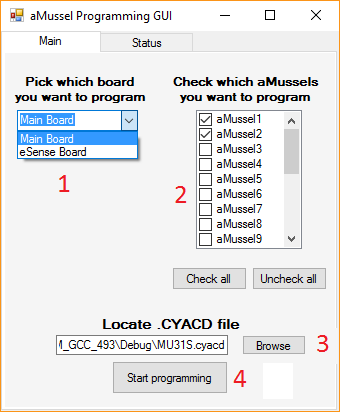
\includegraphics[width=3.8cm]{./figures/programming_gui_main_screen_boards.PNG}}
\label{subflo:windows_programming_application_main}
\hfill
\subfloat[Status screen - Idle]{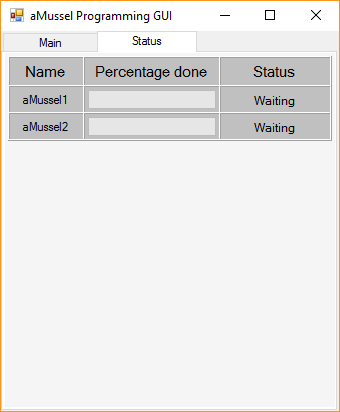
\includegraphics[width=3.8cm]{./figures/programming_gui_status_screen.PNG}}
\hfill
\subfloat[Status screen - Transfering code]{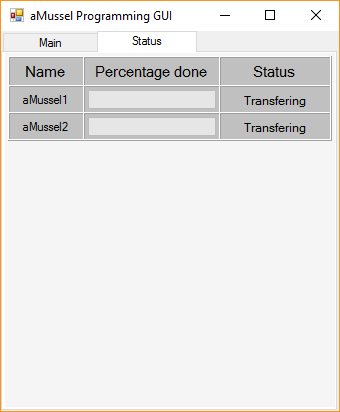
\includegraphics[width=3.8cm]{./figures/programming_gui_status_screen_transfering.PNG}}
%\hfill
\vfill
%\hfill
\subfloat[Status screen - Compiling code]{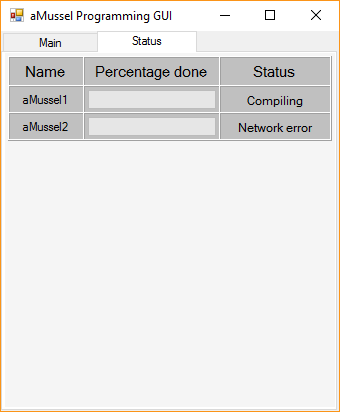
\includegraphics[width=3.8cm]{./figures/programming_gui_status_screen_compiling.PNG}}
\hfill
\subfloat[Status screen - Programming code]{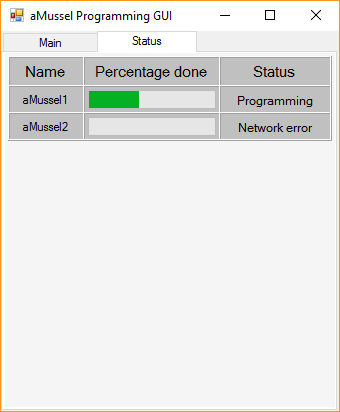
\includegraphics[width=3.8cm]{./figures/programming_gui_status_screen_programming.PNG}}
\hfill
\subfloat[Status screen - Programming done]{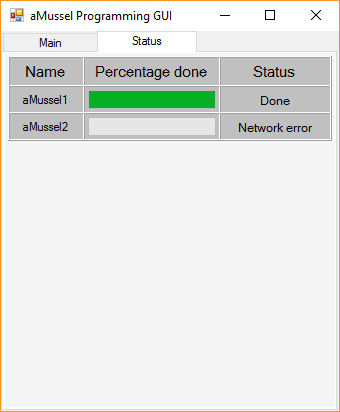
\includegraphics[width=3.8cm]{./figures/programming_gui_status_screen_done.PNG}}
%\hfill
\caption{Windows programming application}
\label{fig:windows_programming_application}
\end{figure}
%TODO change figures to the latest version

To make the process of reprogramming robotic swarm easy, an automated programming application was made.
The application was made in Visual Studio, using the Visual C++ programming language.

The programming procedure is divided in five steps:
\begin{itemize}
\item Choosing a programming configuration
\item Starting the programming procedure
\item Transferring the binary file containing the code
\item Compiling the program on RaspberryPI for programming the PSoC board over I2C
\item Executing the compiled program

\end{itemize}

As shown in \ref{fig:windows_programming_application}a), choosing a programming configuration is split in three steps:
\begin{itemize}
\item Choosing the appropriate board
\item Choosing which aMussels the operator wants to program
\item Choosing the binary file containing the code
\end{itemize}

Before the pressing \textit{Start programming} button in step 2., in the status tab aMussels 1 and 2 are shown to be in waiting mode (\ref{fig:windows_programming_application}b)).
After the programming procedure has started, the status indicator of each aMussel is indicating that the transferring procedure has started (\ref{fig:windows_programming_application}c)).
In case of an unsuccessful file transfer, the status indicator shows "Network error", as seen in aMussel2's status(\ref{fig:windows_programming_application}d)).
The compiling step is shown in \ref{fig:windows_programming_application}d in aMussel1's status.
In the final stage of the programming procedure, the progress bar indicates the percentage of flash memory currently transferred to the PSoC board (\ref{fig:windows_programming_application}e)).
After successful programming, the status indicator of aMussel1 is in the "Done" state and the aMussel should start executing the newly programmed code.

%TODO: transfer obsolete parts to Appendix 
%\subsection{Programming over USB connection (obsolete)}
%
%Setup described in this section enables you to program Main Boards using wired connection (i.e. mini USB cable) Bootloader.
%
%
%\begin{figure}[htb]
%    \centering
%	  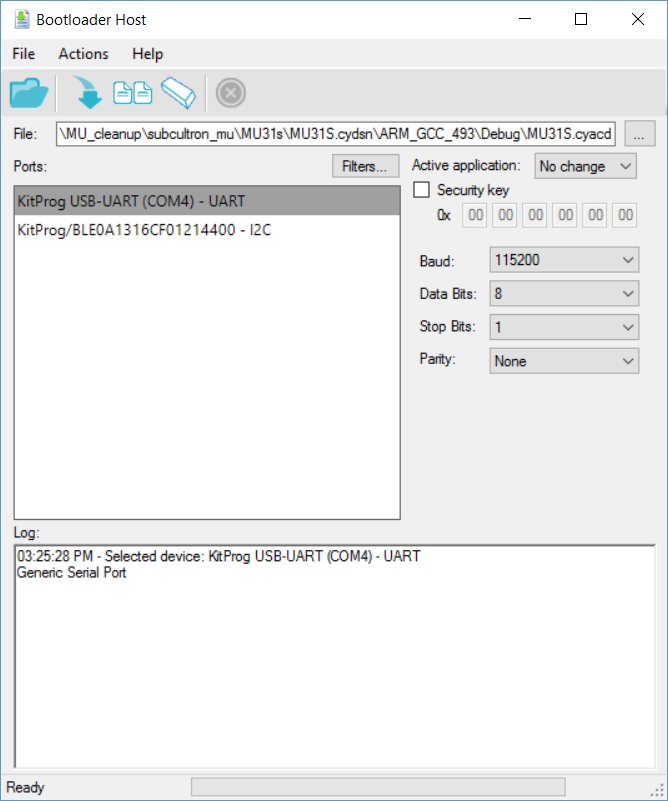
\includegraphics[width=0.6\linewidth]{figures/Bootloader_BLE.PNG}
%	\caption{Setting up Bootloader Host}
%	\label{fig:bootloader_host}
%\end{figure}
%
%Steps:
%\begin{enumerate}
%	\item Connect the MB to your PC via mini USB cable. Make sure all connections to this COM port are closed (stop connections in Docklight).
%	\item Open the project you wish to program in PSoC Creator.
%	\item Go to \texttt{Tools} > \texttt{Bootloader Host}.
%	\item Select the correct COM port and adjust settings to match the ones in Figure \ref{fig:bootloader_host}.
%	\item Click on \texttt{Program} button and wait for the process to execute.
%\end{enumerate}
%
%
%\subsection{Programming over BLE (obsolete)}
%
%The process of programming MB using BLE Bootloader is the same as the one using wired connection Bootloader. The only difference is in the way the connection to the device is established (step 1 in the previous section). For guide on setting up BLE bridge between MB and PC, refer to Chapter \ref{ch:connecting_to_ble}. Bootloader project that needs to be programmed onto the Main Board is \texttt{UART\_Bootloader\_BLE}.
